% Options for packages loaded elsewhere
\PassOptionsToPackage{unicode}{hyperref}
\PassOptionsToPackage{hyphens}{url}
%
\documentclass[
]{article}
\usepackage{lmodern}
\usepackage{amsmath}
\usepackage{ifxetex,ifluatex}
\ifnum 0\ifxetex 1\fi\ifluatex 1\fi=0 % if pdftex
  \usepackage[T1]{fontenc}
  \usepackage[utf8]{inputenc}
  \usepackage{textcomp} % provide euro and other symbols
  \usepackage{amssymb}
\else % if luatex or xetex
  \usepackage{unicode-math}
  \defaultfontfeatures{Scale=MatchLowercase}
  \defaultfontfeatures[\rmfamily]{Ligatures=TeX,Scale=1}
\fi
% Use upquote if available, for straight quotes in verbatim environments
\IfFileExists{upquote.sty}{\usepackage{upquote}}{}
\IfFileExists{microtype.sty}{% use microtype if available
  \usepackage[]{microtype}
  \UseMicrotypeSet[protrusion]{basicmath} % disable protrusion for tt fonts
}{}
\makeatletter
\@ifundefined{KOMAClassName}{% if non-KOMA class
  \IfFileExists{parskip.sty}{%
    \usepackage{parskip}
  }{% else
    \setlength{\parindent}{0pt}
    \setlength{\parskip}{6pt plus 2pt minus 1pt}}
}{% if KOMA class
  \KOMAoptions{parskip=half}}
\makeatother
\usepackage{xcolor}
\IfFileExists{xurl.sty}{\usepackage{xurl}}{} % add URL line breaks if available
\IfFileExists{bookmark.sty}{\usepackage{bookmark}}{\usepackage{hyperref}}
\hypersetup{
  pdftitle={Gestion de Portefeuille},
  pdfauthor={Paul Giraud , Kouamé YAO \& Loïc Turounet},
  hidelinks,
  pdfcreator={LaTeX via pandoc}}
\urlstyle{same} % disable monospaced font for URLs
\usepackage[margin=1in]{geometry}
\usepackage{color}
\usepackage{fancyvrb}
\newcommand{\VerbBar}{|}
\newcommand{\VERB}{\Verb[commandchars=\\\{\}]}
\DefineVerbatimEnvironment{Highlighting}{Verbatim}{commandchars=\\\{\}}
% Add ',fontsize=\small' for more characters per line
\usepackage{framed}
\definecolor{shadecolor}{RGB}{248,248,248}
\newenvironment{Shaded}{\begin{snugshade}}{\end{snugshade}}
\newcommand{\AlertTok}[1]{\textcolor[rgb]{0.94,0.16,0.16}{#1}}
\newcommand{\AnnotationTok}[1]{\textcolor[rgb]{0.56,0.35,0.01}{\textbf{\textit{#1}}}}
\newcommand{\AttributeTok}[1]{\textcolor[rgb]{0.77,0.63,0.00}{#1}}
\newcommand{\BaseNTok}[1]{\textcolor[rgb]{0.00,0.00,0.81}{#1}}
\newcommand{\BuiltInTok}[1]{#1}
\newcommand{\CharTok}[1]{\textcolor[rgb]{0.31,0.60,0.02}{#1}}
\newcommand{\CommentTok}[1]{\textcolor[rgb]{0.56,0.35,0.01}{\textit{#1}}}
\newcommand{\CommentVarTok}[1]{\textcolor[rgb]{0.56,0.35,0.01}{\textbf{\textit{#1}}}}
\newcommand{\ConstantTok}[1]{\textcolor[rgb]{0.00,0.00,0.00}{#1}}
\newcommand{\ControlFlowTok}[1]{\textcolor[rgb]{0.13,0.29,0.53}{\textbf{#1}}}
\newcommand{\DataTypeTok}[1]{\textcolor[rgb]{0.13,0.29,0.53}{#1}}
\newcommand{\DecValTok}[1]{\textcolor[rgb]{0.00,0.00,0.81}{#1}}
\newcommand{\DocumentationTok}[1]{\textcolor[rgb]{0.56,0.35,0.01}{\textbf{\textit{#1}}}}
\newcommand{\ErrorTok}[1]{\textcolor[rgb]{0.64,0.00,0.00}{\textbf{#1}}}
\newcommand{\ExtensionTok}[1]{#1}
\newcommand{\FloatTok}[1]{\textcolor[rgb]{0.00,0.00,0.81}{#1}}
\newcommand{\FunctionTok}[1]{\textcolor[rgb]{0.00,0.00,0.00}{#1}}
\newcommand{\ImportTok}[1]{#1}
\newcommand{\InformationTok}[1]{\textcolor[rgb]{0.56,0.35,0.01}{\textbf{\textit{#1}}}}
\newcommand{\KeywordTok}[1]{\textcolor[rgb]{0.13,0.29,0.53}{\textbf{#1}}}
\newcommand{\NormalTok}[1]{#1}
\newcommand{\OperatorTok}[1]{\textcolor[rgb]{0.81,0.36,0.00}{\textbf{#1}}}
\newcommand{\OtherTok}[1]{\textcolor[rgb]{0.56,0.35,0.01}{#1}}
\newcommand{\PreprocessorTok}[1]{\textcolor[rgb]{0.56,0.35,0.01}{\textit{#1}}}
\newcommand{\RegionMarkerTok}[1]{#1}
\newcommand{\SpecialCharTok}[1]{\textcolor[rgb]{0.00,0.00,0.00}{#1}}
\newcommand{\SpecialStringTok}[1]{\textcolor[rgb]{0.31,0.60,0.02}{#1}}
\newcommand{\StringTok}[1]{\textcolor[rgb]{0.31,0.60,0.02}{#1}}
\newcommand{\VariableTok}[1]{\textcolor[rgb]{0.00,0.00,0.00}{#1}}
\newcommand{\VerbatimStringTok}[1]{\textcolor[rgb]{0.31,0.60,0.02}{#1}}
\newcommand{\WarningTok}[1]{\textcolor[rgb]{0.56,0.35,0.01}{\textbf{\textit{#1}}}}
\usepackage{graphicx}
\makeatletter
\def\maxwidth{\ifdim\Gin@nat@width>\linewidth\linewidth\else\Gin@nat@width\fi}
\def\maxheight{\ifdim\Gin@nat@height>\textheight\textheight\else\Gin@nat@height\fi}
\makeatother
% Scale images if necessary, so that they will not overflow the page
% margins by default, and it is still possible to overwrite the defaults
% using explicit options in \includegraphics[width, height, ...]{}
\setkeys{Gin}{width=\maxwidth,height=\maxheight,keepaspectratio}
% Set default figure placement to htbp
\makeatletter
\def\fps@figure{htbp}
\makeatother
\setlength{\emergencystretch}{3em} % prevent overfull lines
\providecommand{\tightlist}{%
  \setlength{\itemsep}{0pt}\setlength{\parskip}{0pt}}
\setcounter{secnumdepth}{-\maxdimen} % remove section numbering
\usepackage[utf8]{inputenc}
\usepackage{booktabs}
\usepackage{longtable}
\usepackage{array}
\usepackage{multirow}
\usepackage{wrapfig}
\usepackage{float}
\usepackage{colortbl}
\usepackage{pdflscape}
\usepackage{tabu}
\usepackage{threeparttable}
\usepackage{threeparttablex}
\usepackage[normalem]{ulem}
\usepackage{makecell}
\usepackage{xcolor}
\ifluatex
  \usepackage{selnolig}  % disable illegal ligatures
\fi

\title{Gestion de Portefeuille}
\usepackage{etoolbox}
\makeatletter
\providecommand{\subtitle}[1]{% add subtitle to \maketitle
  \apptocmd{\@title}{\par {\large #1 \par}}{}{}
}
\makeatother
\subtitle{TP-3: Modèle à un facteur}
\author{Paul Giraud , Kouamé YAO \& Loïc Turounet}
\date{Version: 26 fév 2022}

\begin{document}
\maketitle

\begin{Shaded}
\begin{Highlighting}[]
\FunctionTok{library}\NormalTok{(xts)}
\FunctionTok{library}\NormalTok{(hornpa)}
\FunctionTok{library}\NormalTok{(lubridate)}
\FunctionTok{library}\NormalTok{(xtable)}
\FunctionTok{library}\NormalTok{(PerformanceAnalytics)}
\FunctionTok{library}\NormalTok{(TTR)}
\FunctionTok{library}\NormalTok{(lubridate)}
\FunctionTok{library}\NormalTok{(roll)}
\FunctionTok{library}\NormalTok{(Hmisc)}
\FunctionTok{library}\NormalTok{(nFactors)}
\FunctionTok{library}\NormalTok{(kableExtra)}
\FunctionTok{library}\NormalTok{(broom)}
\FunctionTok{library}\NormalTok{(quadprog)}
\end{Highlighting}
\end{Shaded}

\hypertarget{donnuxe9es}{%
\section{Données}\label{donnuxe9es}}

\hypertarget{suxe9ries-de-rendement-mensuel-pour-11-valeurs}{%
\subsection{Séries de rendement mensuel pour 11
valeurs:}\label{suxe9ries-de-rendement-mensuel-pour-11-valeurs}}

\begin{Shaded}
\begin{Highlighting}[]
\NormalTok{monthly.ret.file }\OtherTok{\textless{}{-}} \StringTok{"./monthly.ret.rda"}
\FunctionTok{load}\NormalTok{(monthly.ret.file)}
\FunctionTok{index}\NormalTok{(monthly.ret) }\OtherTok{\textless{}{-}} \FunctionTok{floor\_date}\NormalTok{(}\FunctionTok{index}\NormalTok{(monthly.ret), }\StringTok{"month"}\NormalTok{)}
\end{Highlighting}
\end{Shaded}

\hypertarget{matrice-de-covariance-des-rendements}{%
\subsection{Matrice de covariance des
rendements:}\label{matrice-de-covariance-des-rendements}}

\begin{Shaded}
\begin{Highlighting}[]
\FunctionTok{kable}\NormalTok{(}\FunctionTok{cov}\NormalTok{(monthly.ret), }\StringTok{"latex"}\NormalTok{, }\AttributeTok{booktabs=}\NormalTok{T) }\SpecialCharTok{\%\textgreater{}\%}
\FunctionTok{kable\_styling}\NormalTok{(}\AttributeTok{latex\_options=}\FunctionTok{c}\NormalTok{(}\StringTok{"scale\_down"}\NormalTok{, }\StringTok{"HOLD\_position"}\NormalTok{))}
\end{Highlighting}
\end{Shaded}

\begin{table}[H]
\centering
\resizebox{\linewidth}{!}{
\begin{tabular}{lrrrrrrrrrrr}
\toprule
  & AAPL & AMZN & MSFT & F & SPY & QQQ & XOM & MMM & HD & PG & KO\\
\midrule
AAPL & 0.0079015 & 0.0035933 & 0.0028724 & 0.0036506 & 0.0021193 & 0.0033242 & 0.0012183 & 0.0019158 & 0.0012159 & 0.0009073 & 0.0009576\\
AMZN & 0.0035933 & 0.0097937 & 0.0026625 & 0.0025940 & 0.0020258 & 0.0030033 & 0.0011468 & 0.0016726 & 0.0016066 & 0.0003831 & 0.0013968\\
MSFT & 0.0028724 & 0.0026625 & 0.0044949 & 0.0032132 & 0.0017774 & 0.0022969 & 0.0009976 & 0.0012898 & 0.0015753 & 0.0007414 & 0.0011363\\
F & 0.0036506 & 0.0025940 & 0.0032132 & 0.0226257 & 0.0032869 & 0.0034954 & 0.0017697 & 0.0034663 & 0.0032642 & 0.0014660 & 0.0014993\\
SPY & 0.0021193 & 0.0020258 & 0.0017774 & 0.0032869 & 0.0017549 & 0.0019207 & 0.0012159 & 0.0016906 & 0.0015105 & 0.0008284 & 0.0009008\\
\addlinespace
QQQ & 0.0033242 & 0.0030033 & 0.0022969 & 0.0034954 & 0.0019207 & 0.0025159 & 0.0010479 & 0.0016973 & 0.0016125 & 0.0007561 & 0.0008650\\
XOM & 0.0012183 & 0.0011468 & 0.0009976 & 0.0017697 & 0.0012159 & 0.0010479 & 0.0025213 & 0.0015076 & 0.0008121 & 0.0006409 & 0.0007365\\
MMM & 0.0019158 & 0.0016726 & 0.0012898 & 0.0034663 & 0.0016906 & 0.0016973 & 0.0015076 & 0.0032027 & 0.0016559 & 0.0009968 & 0.0008642\\
HD & 0.0012159 & 0.0016066 & 0.0015753 & 0.0032642 & 0.0015105 & 0.0016125 & 0.0008121 & 0.0016559 & 0.0037458 & 0.0005615 & 0.0005566\\
PG & 0.0009073 & 0.0003831 & 0.0007414 & 0.0014660 & 0.0008284 & 0.0007561 & 0.0006409 & 0.0009968 & 0.0005615 & 0.0018508 & 0.0009004\\
\addlinespace
KO & 0.0009576 & 0.0013968 & 0.0011363 & 0.0014993 & 0.0009008 & 0.0008650 & 0.0007365 & 0.0008642 & 0.0005566 & 0.0009004 & 0.0019550\\
\bottomrule
\end{tabular}}
\end{table}

\hypertarget{rendement-moyen-mensuel}{%
\subsection{Rendement moyen mensuel}\label{rendement-moyen-mensuel}}

\begin{Shaded}
\begin{Highlighting}[]
\FunctionTok{kbl}\NormalTok{(}\FunctionTok{colMeans}\NormalTok{(monthly.ret), }\AttributeTok{format=}\StringTok{"latex"}\NormalTok{, }\AttributeTok{booktabs=}\NormalTok{T,}
    \AttributeTok{col.names=}\FunctionTok{c}\NormalTok{(}\StringTok{"Rendement"}\NormalTok{), }\AttributeTok{caption=}\StringTok{"Rendement moyen mensuel"}\NormalTok{) }\SpecialCharTok{\%\textgreater{}\%}
    \FunctionTok{kable\_styling}\NormalTok{(}\AttributeTok{latex\_options=}\StringTok{"HOLD\_position"}\NormalTok{)}
\end{Highlighting}
\end{Shaded}

\begin{table}[H]

\caption{\label{tab:unnamed-chunk-3}Rendement moyen mensuel}
\centering
\begin{tabular}[t]{lr}
\toprule
  & Rendement\\
\midrule
AAPL & 0.0254037\\
AMZN & 0.0298355\\
MSFT & 0.0151864\\
F & 0.0115177\\
SPY & 0.0075856\\
\addlinespace
QQQ & 0.0122593\\
XOM & 0.0016595\\
MMM & 0.0079299\\
HD & 0.0151356\\
PG & 0.0073821\\
\addlinespace
KO & 0.0100164\\
\bottomrule
\end{tabular}
\end{table}

\hypertarget{taux-sans-risque}{%
\subsection{Taux sans risque}\label{taux-sans-risque}}

Le taux sans risque mensuel est obtenu de la Réserve Fédérale US. A
diviser par 12 pour être cohérent avec les rendement des titres.

\begin{Shaded}
\begin{Highlighting}[]
\NormalTok{tmp }\OtherTok{\textless{}{-}} \FunctionTok{read.csv}\NormalTok{(}\StringTok{"DP\_LIVE\_01032020211755676.csv"}\NormalTok{, }\AttributeTok{header=}\ConstantTok{TRUE}\NormalTok{, }\AttributeTok{sep=}\StringTok{";"}\NormalTok{)[, }\FunctionTok{c}\NormalTok{(}\StringTok{"TIME"}\NormalTok{, }\StringTok{"Value"}\NormalTok{)]}
\NormalTok{dt }\OtherTok{\textless{}{-}} \FunctionTok{ymd}\NormalTok{(}\FunctionTok{paste}\NormalTok{(tmp}\SpecialCharTok{$}\NormalTok{TIME, }\StringTok{"{-}01"}\NormalTok{, }\AttributeTok{sep=}\StringTok{""}\NormalTok{))}
\NormalTok{rf\_rate }\OtherTok{\textless{}{-}} \FunctionTok{xts}\NormalTok{((tmp}\SpecialCharTok{$}\NormalTok{Value}\SpecialCharTok{/}\FloatTok{100.0}\NormalTok{)}\SpecialCharTok{/}\DecValTok{12}\NormalTok{, dt)}
\FunctionTok{colnames}\NormalTok{(rf\_rate) }\OtherTok{\textless{}{-}} \StringTok{"Rf"}
\NormalTok{monthly.ret}\FloatTok{.2} \OtherTok{\textless{}{-}} \FunctionTok{merge.xts}\NormalTok{(monthly.ret, rf\_rate, }\AttributeTok{join=}\StringTok{"inner"}\NormalTok{)}
\end{Highlighting}
\end{Shaded}

\begin{figure}
\centering
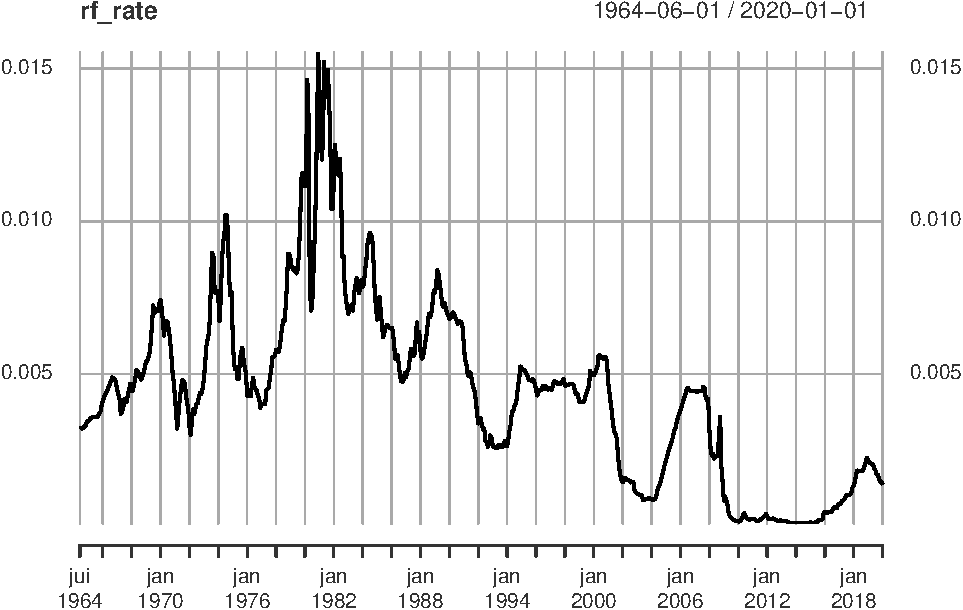
\includegraphics{TP-3_files/figure-latex/unnamed-chunk-5-1.pdf}
\caption{taux sans risque mensuel}
\end{figure}

\hypertarget{estimation-dun-moduxe8le-uxe0-un-facteur}{%
\section{Estimation d'un modèle à un
facteur}\label{estimation-dun-moduxe8le-uxe0-un-facteur}}

\begin{itemize}
\tightlist
\item
  Utiliser l'indice SPY comme proxy pour le marché et estimer pour
  chaque titre le modèle:
\end{itemize}

\[
R_i(t) - R_f(t) = \alpha + \beta (R_M(t) - R_f(t)) + \epsilon(t)
\] en utilisant la fonction \texttt{lm}. - Placer chaque titre sur un
diagramme rendement/beta et calculer par regression la droite de marché
des titres risqués. - En déduire les titres qui, selon ce modèle,
\emph{semblent} chers et ceux qui semblent sous-évalués.

\begin{Shaded}
\begin{Highlighting}[]
\NormalTok{names }\OtherTok{\textless{}{-}} \FunctionTok{colnames}\NormalTok{(monthly.ret}\FloatTok{.2}\NormalTok{)}
\NormalTok{df }\OtherTok{\textless{}{-}} \FunctionTok{data.frame}\NormalTok{(}\FunctionTok{setNames}\NormalTok{(}\FunctionTok{rep}\NormalTok{(}\FunctionTok{list}\NormalTok{(}\DecValTok{0}\NormalTok{), }\FunctionTok{length}\NormalTok{(names)), names))}
\NormalTok{number.assets }\OtherTok{=} \FunctionTok{dim}\NormalTok{(monthly.ret}\FloatTok{.2}\NormalTok{)[}\DecValTok{2}\NormalTok{]}

\NormalTok{ret.proxy.spy }\OtherTok{\textless{}{-}}\NormalTok{ monthly.ret}\FloatTok{.2}\SpecialCharTok{$}\NormalTok{SPY }\SpecialCharTok{{-}}\NormalTok{ monthly.ret}\FloatTok{.2}\SpecialCharTok{$}\NormalTok{Rf}
\ControlFlowTok{for}\NormalTok{ (i }\ControlFlowTok{in} \DecValTok{1}\SpecialCharTok{:}\NormalTok{number.assets)\{}
\NormalTok{  ret }\OtherTok{\textless{}{-}}\NormalTok{ monthly.ret}\FloatTok{.2}\NormalTok{[,i] }\SpecialCharTok{{-}}\NormalTok{ monthly.ret}\FloatTok{.2}\SpecialCharTok{$}\NormalTok{Rf}
\NormalTok{  linear\_model }\OtherTok{\textless{}{-}} \FunctionTok{lm}\NormalTok{(ret }\SpecialCharTok{\textasciitilde{}}\NormalTok{ ret.proxy.spy)}
\NormalTok{  df[}\DecValTok{1}\SpecialCharTok{:}\DecValTok{2}\NormalTok{,i] }\OtherTok{\textless{}{-}}\NormalTok{ linear\_model}\SpecialCharTok{$}\NormalTok{coefficients}
\NormalTok{\}}
\FunctionTok{row.names}\NormalTok{(df) }\OtherTok{\textless{}{-}} \FunctionTok{c}\NormalTok{(}\StringTok{"alpha"}\NormalTok{, }\StringTok{"beta"}\NormalTok{)}
\end{Highlighting}
\end{Shaded}

\begin{Shaded}
\begin{Highlighting}[]
\FunctionTok{kable}\NormalTok{(df, }\StringTok{"latex"}\NormalTok{, }\AttributeTok{booktabs=}\NormalTok{T, }\AttributeTok{caption=}\StringTok{"Alpha and Beta for each asset"}\NormalTok{) }\SpecialCharTok{\%\textgreater{}\%}
\FunctionTok{kable\_styling}\NormalTok{(}\AttributeTok{latex\_options=}\FunctionTok{c}\NormalTok{(}\StringTok{"scale\_down"}\NormalTok{, }\StringTok{"HOLD\_position"}\NormalTok{))}
\end{Highlighting}
\end{Shaded}

\begin{table}[H]

\caption{\label{tab:unnamed-chunk-7}Alpha and Beta for each asset}
\centering
\resizebox{\linewidth}{!}{
\begin{tabular}[t]{lrrrrrrrrrrrr}
\toprule
  & AAPL & AMZN & MSFT & F & SPY & QQQ & XOM & MMM & HD & PG & KO & Rf\\
\midrule
alpha & 0.0167401 & 0.0212874 & 0.0073307 & -0.0008543 & 0 & 0.0039254 & -0.0031066 & 0.0007451 & 0.0080456 & 0.0034204 & 0.0056304 & 0\\
beta & 1.1948376 & 1.1465481 & 1.0148488 & 1.8508513 & 1 & 1.0959372 & 0.6751296 & 0.9608010 & 0.8746106 & 0.4693130 & 0.5136098 & 0\\
\bottomrule
\end{tabular}}
\end{table}

Ainsi, nous pouvons observer d'après la Table 2, que le alpha du SPY est
nul et que son beta est égale à 1. Cela nous permet de valider nos
calculs de alpha et beta, en effet, le SPY a été choisi comme proxy pour
le marché.

\begin{verbatim}
## 
## Call:
## lm(formula = df.ret.beta$return ~ df.ret.beta$beta)
## 
## Coefficients:
##      (Intercept)  df.ret.beta$beta  
##         0.002194          0.010195
\end{verbatim}

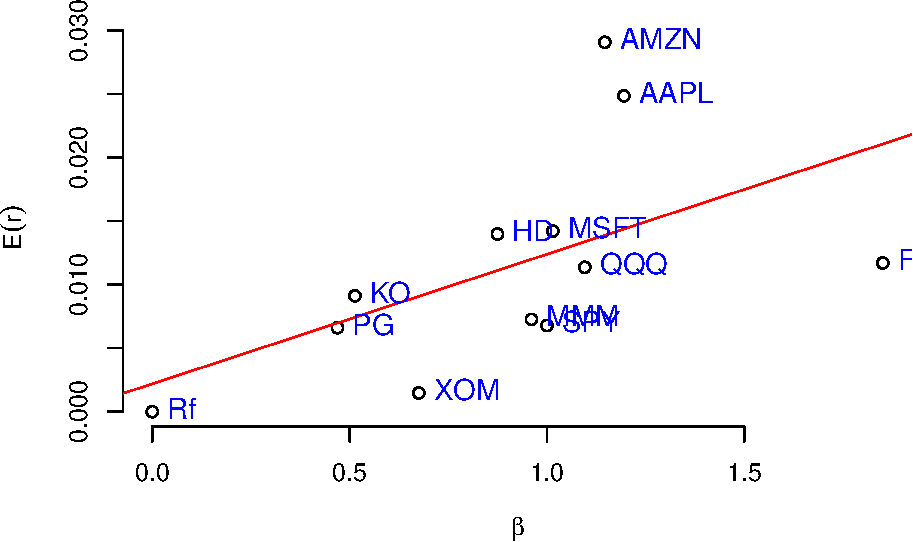
\includegraphics{TP-3_files/figure-latex/unnamed-chunk-8-1.pdf}

Résultats :

\begin{itemize}
\tightlist
\item
\item
\item
\item
\item
\item
\item
\item
\item
\end{itemize}

Est-ce que ces mesures de cherté relative vous semble correctes? Essayez
de mesurer la robustesse de ce calcul en estimant le modèles sur des
sous-intervalles de temps.

Présentez vos résultats de manière synthétique.

\end{document}
